\section{Organizzazione dei dati e validazione}
\label{sec:data}

\begin{wrapfigure}{r}{0.34\textwidth}
  \vspace{-1.2em}
  \centering
  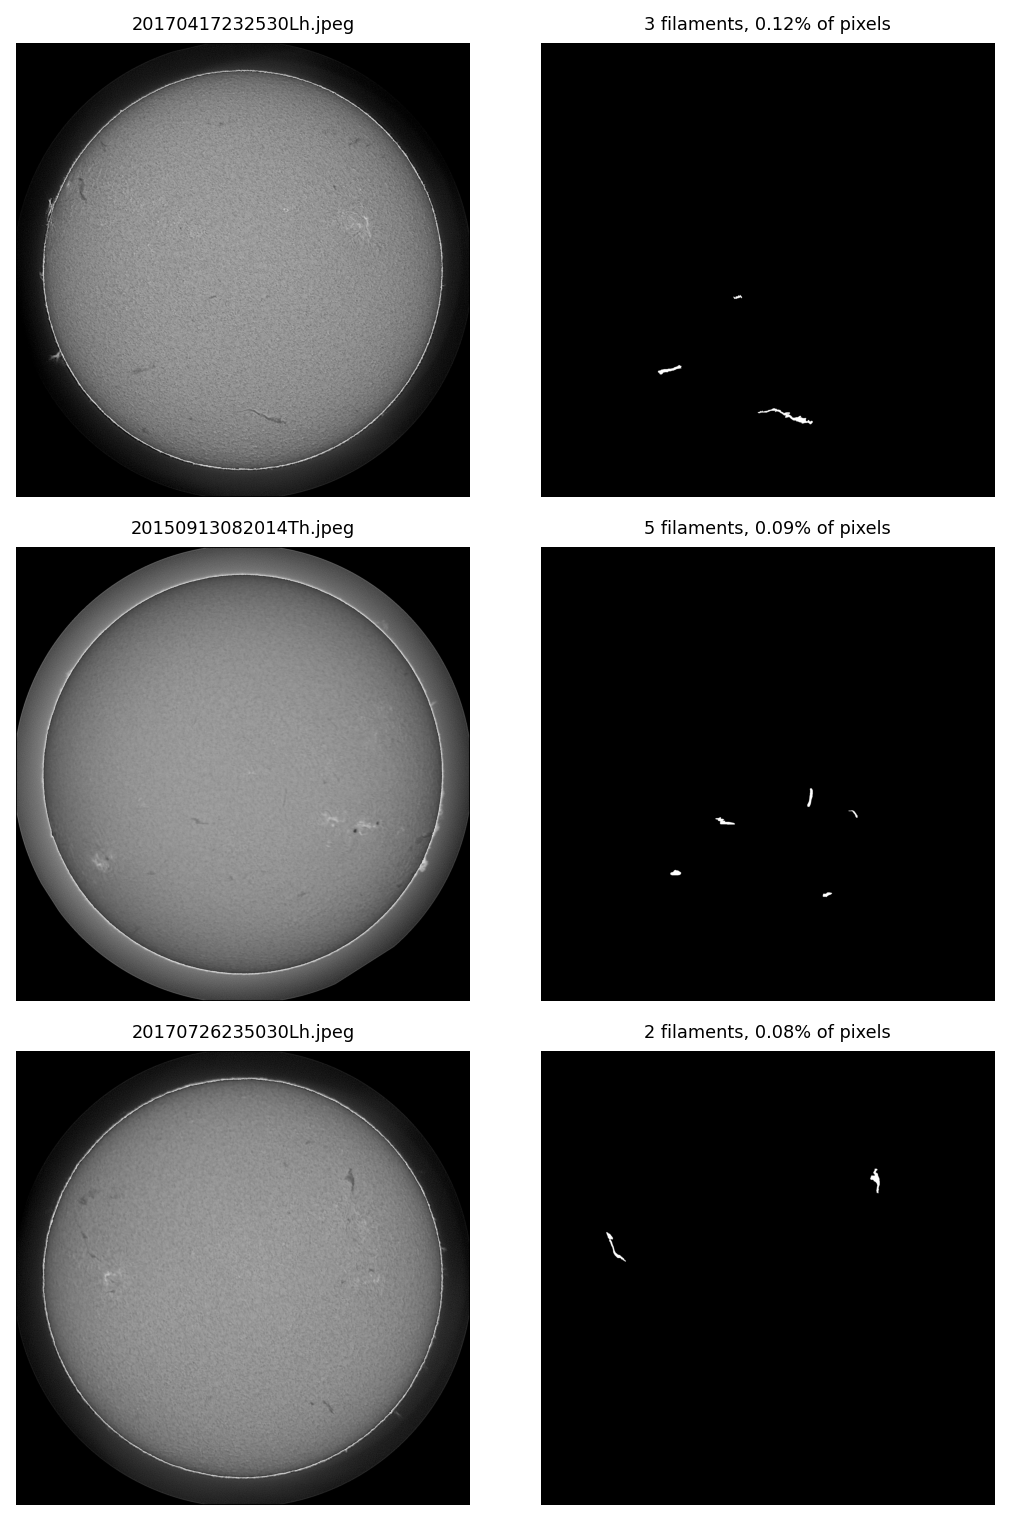
\includegraphics[width=0.32\textwidth]{figures/dataset_examples_13.png}
  \caption{Esempi usati per controllare il contrasto delle immagini e la variabilità
  delle annotazioni.}
  \label{fig:dataset}
  \vspace{-1em}
\end{wrapfigure}

I dati annotati contengono 707 osservazioni diverse ma 1154 record di annotazione.
Diverse osservazioni sono state annotate da due o tre esperti. Una suddivisione casuale
dei singoli record avrebbe quindi potuto assegnare annotazioni della stessa immagine sia
al training sia alla validazione. In tal caso, il modello sarebbe stato valutato su
immagini già incontrate durante l'addestramento, con una conseguente sovrastima delle
prestazioni. Per evitare questa forma di data leakage, ho effettuato lo split a livello
di file, assegnando tutte le annotazioni della stessa osservazione a un unico insieme.

Lo split finale usa il seed 22 e contiene 601 file di training e 106 di validazione,
corrispondenti a 985 e 169 record di annotazione. Il test set separato di Kaggle viene
usato solo dal notebook di inferenza. Le appartenenze esatte sono salvate in
\texttt{split\_seed22.csv}, quindi il validation set riportato può essere ricostruito.

Le maschere contengono 8199 poligoni di filamenti e il foreground occupa solo circa lo
0.4\% di un'immagine. L'area mediana di un'istanza alla risoluzione nativa è di circa
1230 pixel. Nelle osservazioni con più annotazioni, il Dice medio tra coppie di
annotatori è circa 0.62. Questo valore non definisce un limite superiore umano, ma mostra
che alcuni errori apparenti della previsione possono dipendere anche dalle differenze tra
gli annotatori.

La validazione è stata usata per scegliere il checkpoint, confrontare gli esperimenti e
selezionare le impostazioni finali dell'output. Il riuso dello stesso split può rendere
ottimistico il punteggio finale; per questo considero con cautela le differenze piccole.
